\documentclass{article}

% Language setting
% Replace `english' with e.g. `spanish' to change the document language
\usepackage[english]{babel}

% Set page size and margins
% Replace `letterpaper' with `a4paper' for UK/EU standard size
\usepackage[letterpaper,top=2cm,bottom=2cm,left=3cm,right=3cm,marginparwidth=1.75cm]{geometry}

% Useful packages
\usepackage{amsmath} % assumes amsmath package installed
\usepackage{amssymb}  % assumes amsmath package installed
\usepackage{graphicx}
\graphicspath{{./Figures/}}
\usepackage[listofformat=subsimple, caption=false,font=footnotesize]{subfig}
\usepackage{tikz}
\usepackage[colorlinks=true, allcolors=blue]{hyperref}

\title{Object Reorientation with Help of Environment Contact
Project Report}
\author{Maede Boroji, Vahid Danesh}
\date{}
\begin{document}
\maketitle

\begin{abstract}
In this project, we utilized a Tabletop Franka Panda robot to reorient various fallen objects, including cuboids, cylinders, and a mustard bottle. 
%We assumed complete knowledge of the objects' properties, such as dimensions and edges. 
We assumed that the objects' dimensions and initial configurations lie within the robot’s reachable workspace, and that the robot is capable of performing the necessary manipulations, including solving the inverse kinematics, from those initial poses. 
In each scene, the initial configurations of the objects were randomly assigned. Using the adapter available in \texttt{genesis-adapter}, the geometric features—such as size, edges and vertices—were extracted from Genesis API, from which all necessary parameters for motion execution were derived.
This allows us to construct the screw axis which the object will be manipulated about that axis.
Moreover, we explored an extension involving rotational slippage at the grasp point to allow upright manipulation while maximizing manipulability.
All simulations were performed in the Genesis-AI physics-based simulator and we were able to reorient objects in multiple simulations (total of three objects in each scene) with a 96\% success rate. 
%This approach enables manipulation of heavy objects by leveraging environmental contact rather than relying solely on grasping. If time permits, we will also explore an extension involving rotational slippage at the grasp point to allow upright manipulation while maximizing manipulability.
\end{abstract}

\section{Introduction}

In general, any rigid body displacement can be expressed as a rotation $\theta \in \mathbb{R}$ about a screw axis $\mathcal{S}$ followed by a translation $d \in \mathbb{R}$ along the axis. By representing the screw axis $\mathcal{S}$ by a unit vector $\boldsymbol{u} \in \mathbb{R}^3$ along the axis and an arbitrary point $\boldsymbol{r} \in \mathbb{R}^3$ on the axis, the screw parameters, using Plücker coordinates, are defined as $(\theta,d,\boldsymbol{u},\boldsymbol{m})$, where $\boldsymbol{m}= \boldsymbol{r} \times \boldsymbol{u} \in \mathbb{R}^3$. Therefore, the screw motions can be efficiently expressed by the dual quaternions as $ D_T = Q_R + \epsilon \frac{1}{2} Q_P Q_R =( \cos\frac{\theta}{2} + \boldsymbol{u}\sin\frac{\theta}{2}) + \epsilon\left(-\frac{d}{2}\sin\frac{\theta}{2}+\sin\frac{\theta}{2}\boldsymbol{m}+\frac{d}{2}\cos\frac{\theta}{2}\boldsymbol{u}\right)$. In our case which is a \texttt{constant} screw motion, $\boldsymbol{u}$ and $\boldsymbol{m}$ remains constant and only $\theta$ changes.  The smooth path in $SE(3)$ provided by the ScLERP is derived by $D(s) = D_1D_{12}^{s}$, where $s \in [0, 1]$ is a scalar path parameter and $D_{12}$ is the transformation of $\mathcal{C}_2$ with respect to $\mathcal{C}_1$. $D_{12}^ {s}$ can be computed using $D_{12}^{s} = \left(\cos \frac{s \theta}{2}, \sin \frac{s\theta}{2}\boldsymbol{u}\right) + \epsilon \left(- \frac{s d}{2} \sin \frac{s \theta}{2}, \frac{s d}{2}\cos \frac{s \theta}{2} \boldsymbol{u} + \sin \frac{s \theta}{2} \boldsymbol{m}\right)$ after extracting the screw parameters $\boldsymbol{u}$, $\boldsymbol{m}$, $\theta$, $d$ from $D_{12}$.

If $\mathcal{C}_1$ and $\mathcal{C}_2$ have a contact edge in common, the final pose can be achieved by pivoting the object about the common edge, as shown in Fig.~\ref{Fig:SRP}. 

\begin{figure}[!htbp]
    \centering
    {\includegraphics[scale=0.76]{Figures/T.pdf}\label{Fig:SRP_T}}
    \caption{Manipulating cuboid-shape objects by exploiting the environment contact, through pivoting about an edge. Courtesy of image~\cite{Fakhari2020MotionAF}}
\label{Fig:SRP}
\end{figure}
\subsection{Motivation}
In conventional object reorientation, when rotational slippage is not permitted at the grasp point, the object becomes rigidly coupled to the robot's end-effector. This rigid coupling means that any rotation applied to the object must be executed by the robot's joints, creating several limitations. First, as the object approaches its final upright position during pivoting, the end-effector is forced to move closer to the ground, often resulting in potential collisions with the environment as illustrated in Fig~\ref{Fig:CubeCylinder_Sclerp}. Second, this constraint significantly restricts the robot's workspace and manipulability, as the robot must maintain specific wrist orientations throughout the entire motion, limiting the range of feasible object configurations that can be successfully reoriented. Additionally, the rigid coupling requires the robot to execute more complex joint movements, which can limit robot's overall 
manipulability and dexterity during the task execution. 
\begin{figure}[!htbp]
\centering
    \subfloat[]{\includegraphics[scale=0.205]{Figures/Cube_Sclerp1.jpg}} \quad \,
    \subfloat[]{\includegraphics[scale=0.21]{Figures/Cube_sclerp2.jpg}} \quad \,
    \subfloat[]{\includegraphics[scale=0.22]{Figures/Cylinder_sclerp1.jpg}}\quad \,
    \subfloat[]{\includegraphics[scale=0.2]{Figures/Cylinder_sclerp2.jpg}}
    \caption{Object reorientation without rotational slippage: A cube is reoriented from its initial pose $\mathcal{C}_O$ (a) to the goal pose $\mathcal{C}_F$ (b), and a cylinder from its initial pose (c) to its goal pose (d).}
\label{Fig:CubeCylinder_Sclerp}
\end{figure}

This motivates us to explore a new method in which the manipulator induces object motion through rotational slippage at the grasp point while maintaining a fixed (or nearly fixed) end-effector orientation. This enables more dexterous manipulation while maximizing the robot’s manipulability. 

\section{Method}
We used the Franka Emika Panda robot and simulate it in a physics-based simulator, Genesis-AI~\cite{Genesis}.
The object set include cuboids, cylinders, and a mustard bottle. All objects initially lied in random arbitrary poses on a tabletop and the goal was to reorient them to an upright configuration.
All manipulated objects were defined within Genesis-AI available models.

\subsection{Screw parameters}
All screw motion parameters were derived by fitting an Oriented Bounding Box (OBB) to the object and extracting its eight vertices and twelve edges. From these, only the edges that are in contact with the ground and can fit within the robot’s gripper are retained. There are always at least two candidate edges suitable for pivoting, and the user can specify which edge to pivot around. By default, the edge that is farthest from the robot’s base is selected.
After determining the screw motion parameters, the grasp pose must be computed. The grasp location lies on the side of the object opposite to the edge where the screw parameters are defined. Once the grasp pose is established, the final pose of the gripper can be calculated using the object's current pose and the screw parameters. With both the current and desired poses represented as dual quaternions, Screw Linear Interpolation (ScLERP) is then performed using pytransform3d package~\cite{Fabisch2019}. Moreover time scaling of the screw motion planner could be set as linear, cubic or quintic.
Here is a brief description of some of the most important functions/adapters in our project:
\subsubsection*{Adapters}
\begin{itemize}
    \item \textbf{GenesisAdapter}: Provides an interface to the Genesis physics engine's geometry representation. It extracts geometric features like size, edges, and vertices from objects in the simulation environment, which are essential for motion planning. The adapter handles coordinate frame conversions and methods to control robot's position and velocity.
    \item \textbf{ScrewMotionPlanner}: Implements the core manipulation planning functionality. It computes screw axes for object manipulation and generates trajectories that allow the robot to reorient objects. The planner supports different time scaling methods (linear, cubic, quintic) and can incorporate rotational slippage.
    \item \textbf{RobotController}: Manages robot motion execution, including grasp positioning, manipulation sequences, and end-effector control. 
\end{itemize}
\subsection{Rotational slippage}
The robot originally has 9 degrees of freedom, 7 from the arm and base and 2 prismatic degrees of freedom from the gripper fingers.
For rotational slippage, we modified the robot's XML model in two ways. First, we added two hinges (revolute joints) directly to the robot's fingers to eliminate torsional friction between the robot's fingers and the grasped object. Second, we defined a virtual revolute joint at the center of the robot's fingers. This virtual finger joint serves as the primary mechanism for controlled rotational slippage during manipulation. The inverse kinematics solver was adapted accordingly to account for these additional degrees of freedom when planning motions.

Incorporating rotational slippage into the screw motion significantly improved the robot's manipulability, allowing it to reorient objects in configurations that were previously infeasible. This can be validated during experiments by adding a hinge joint to the robot's fingers, which enables controlled rotational movement at the grasp point. Figure~\ref{Fig:Rotational_slippage} illustrates an example of a cylinder being reoriented both with and without the use of rotational slippage. As shown, the dexterity and manipulability of the robot significantly increases with rotational slippage at the fingers level, enabling more complex object reorientation tasks to be completed successfully.

\begin{figure}[!htbp]
\centering
    \subfloat[]{\includegraphics[scale=0.35]{Figures/cyl_1.jpg}} \quad \,
    \subfloat[]{\includegraphics[scale=0.355]{Figures/cyl_2.jpg}} \\
    \subfloat[]{\includegraphics[scale=0.25]{Figures/cyl_3.png}} \quad \,
    \subfloat[]{\includegraphics[scale=0.245]{Figures/cyl_4.png}}
    \caption{A cylinder is reoriented without rotational slippage from its initial pose (a) to the maximum reach pose (b), and the same cylinder is reoriented with rotational slippage from its initial pose (c) to its goal pose (d).}
\label{Fig:Rotational_slippage}
\end{figure}

\subsection{Pipeline}
In this model-based control system, the robot begins from a ready configuration and the objects' positions and orientations are initialized randomly within the robot workspace. The object poses are obtained directly from the simulator (no perception module is needed).

A collision-aware RRTConnect motion planner with trajectory smoothing is used to generate feasible paths for the end-effector. This planner creates collision-free trajectories for the approach phase (to grasp the object), while respecting joint position and velocity limits.

\begin{center}
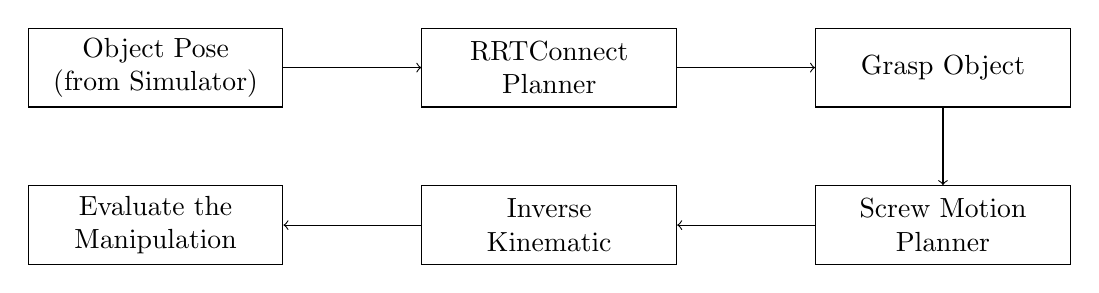
\begin{tikzpicture}[node distance=5cm, auto]
    \node (pose) [draw, rectangle, align=center, text width=3cm, minimum height=1cm] {Object Pose\\(from Simulator)};
    \node (rrt1) [draw, rectangle, right of=pose, align=center, text width=3cm, minimum height=1cm] {RRTConnect\\Planner};
    \node (grasp) [draw, rectangle, right of=rrt1, align=center, text width=3cm, minimum height=1cm] {Grasp Object};
    \node (planner) [draw, rectangle, below of=grasp, align=center, text width=3cm, node distance=2cm, minimum height=1cm] {Screw Motion\\ Planner};
    \node (ik) [draw, rectangle, left of=planner, align=center, text width=3cm, minimum height=1cm] {Inverse\\Kinematic};
    \node (evaluate) [draw, rectangle, left of=ik, align=center, text width=3cm, minimum height=1cm] {Evaluate the \\ Manipulation};

    \draw[->] (pose) -- (rrt1);
    \draw[->] (rrt1) -- (grasp);
    \draw[->] (grasp) -- (planner);
    \draw[->] (planner) -- (ik);
    \draw[->] (ik) -- (evaluate);
\end{tikzpicture}
\end{center}

The RRTConnect planning blocks in the pipeline convert the desired Cartesian space trajectories into smooth, feasible joint space trajectories. The resulting paths are then post-processed with a trajectory smoothing algorithm to eliminate unnecessary jerky motions. After the screw motion planner generates the task space trajectory, we used inverse kinematic to solve for the corresponding joint configurations. This translation from task space to joint space ensures the robot can physically execute the planned screw motion. 

\section{Results}
\subsection{Evaluation metric}
To evaluate how closely the object reaches its target pose, we compared the current pose of the object to its goal. The translational error is extracted directly from the linear displacement, and rotational error is computed using the axis-angle representation.
The success rate is then calculated by combining normalized translational and angular errors into a percentage score, giving an overall measure of how accurately the object was reoriented. A higher success rate indicates better alignment with the target pose. In our simulations, we achieved overall success rates of 94\%, 95\%, and 98\% for reorienting cylinders, bottles, and cubes, respectively, across a range of variable initial poses.
\begin{figure}[!htbp]
\centering
    \subfloat[]{\includegraphics[scale=0.16]{Figures/before.png}} \quad \,
    \subfloat[]{\includegraphics[scale=0.16]{Figures/after.png}} 
    \caption{Reorientation of a cube, cylinder and a mustard bottle with rotational slippage from their initial pose (a) to the goal pose (b).}
\label{Fig:Reoriantion}
\end{figure}

\subsection{Future Work}

A significant advantage of the Genesis-AI framework is its capability to perform batch simulations, allowing multiple scenarios to be evaluated simultaneously. All methods developed in our project are designed to be compatible with this batch simulation functionality, which can dramatically accelerate testing and validation of manipulation strategies across diverse scenarios.

\begin{figure}[!htbp]
\centering
\includegraphics[width=0.9\textwidth]{Figures/batch_simulation.png}
\caption{Batch simulation in Genesis showing parallel execution of object reorientation tasks across different environments.}
\label{Fig:BatchSimulation}
\end{figure}

Currently, the \texttt{plan\_path} methods from Genesis are not fully compatible with batched simulation. Future work will focus on extending other planning methods to support batch operations, enabling parallel computation of motion plans across multiple environments. 

Additionally, we plan to integrate perception-based grasp planning algorithms that can better account for object geometry and physical properties. The integration of learning-based approaches alongside our model-based methods also presents an exciting direction for future research.

\section{Conclusion}

Our evaluation across multiple trials showed consistent performance with a 96\% success rate in achieving the target upright poses. The rotational slippage approach significantly improved manipulability compared to conventional fixed-grasp approaches, allowing successful manipulation of objects in configurations that would otherwise be kinematically challenging.

All codes are accessible in our \href{https://github.com/VahidDanesh/pandaSim}{GitHub repository}. The repository includes the complete implementation, example notebooks, and utilities for reproducing our results. 

Video recordings of the manipulation sequences are available in the \texttt{examples/videos} directory of the repository, showing the execution of the pipeline across different object types.


\bibliographystyle{ieeetr}
\bibliography{references}
\end{document}